\documentclass[12pt,a4paper]{article}
\usepackage[T1]{fontenc}
\usepackage[utf8]{inputenc}
\usepackage{mathptmx}
\usepackage[left=0.95in,right=0.95in,top=0.8in,bottom=0.8in,headheight=15pt,headsep=12pt]{geometry}
\usepackage{graphicx,array,tabularx,caption}
\usepackage{titlesec,fancyhdr,microtype}
\usepackage[hidelinks]{hyperref}
\hypersetup{pdftitle={Implementation of Rate-Limited Sender Functionality in picoquic},
  pdfauthor={Aryan Bokolia, Affan Arshad, Soumyadeep Raj, Kevin Shiju George, Aryan Palimkar}}
\urlstyle{same}
\setlength{\parindent}{0pt}
\setlength{\parskip}{0.45em}
\setlength{\emergencystretch}{3em}
\titleformat{\section}{\fontsize{16}{19}\selectfont\bfseries}{}{0pt}{}
\titleformat{\subsection}{\fontsize{13}{16}\selectfont\bfseries}{}{0pt}{}
\titlespacing*{\section}{0pt}{0.6em}{0.7em}
\titlespacing*{\subsection}{0pt}{0.65em}{0.4em}
\captionsetup{font=small,labelfont=bf,justification=centering,hypcap=false}
\pagestyle{fancy}
\fancyhf{}
\fancyhead[R]{\small Rate-Limited Increase in picoquic}
\fancyfoot[C]{\thepage}
\renewcommand{\headrulewidth}{0.4pt}
\renewcommand{\footrulewidth}{0pt}
\begin{document}
\thispagestyle{empty}
\begin{center}
\vspace*{1.25cm}
{\Large\bfseries OSNT Mini-Project Report\par}
\vspace{0.3cm}
{\large Project \#16\par}
\vspace{0.8cm}
\rule{0.9\linewidth}{0.9pt}\par
\vspace{0.55cm}
{\fontsize{23}{28}\selectfont\bfseries Implementation of Rate-Limited Sender Functionality in the picoquic Library\par}
\vspace{0.35cm}
{\large CUBIC congestion control for QUIC\par}
\vspace{0.55cm}
\rule{0.9\linewidth}{0.45pt}\par
\vspace{1.3cm}
{\large\bfseries Project team\par}
\vspace{0.35cm}
{\large
\renewcommand{\arraystretch}{1.3}
\begin{tabular}{c}
Aryan Bokolia\\
Affan Arshad\\
Soumyadeep Raj\\
Kevin Shiju George\\
Aryan Palimkar
\end{tabular}\par}
\vfill
{\large 9 November 2026\par}
\vspace{1.2cm}
\end{center}
\clearpage
\section*{Abstract}
\label{sec:abstract}
This project implements Rate-Limited Increase (RLI) as an option for CUBIC in picoquic. RLI uses the largest recorded flight size on each path to cap congestion-window growth. A window reduction starts a new flight-size history. We compared original CUBIC and CUBIC with RLI using Linux network namespaces on Ubuntu. The workloads included a fixed-rate stream, bulk transfers, and competing connections on a shared bottleneck.

With a fixed application rate, RLI grew the window to its slow-start limit while throughput stayed essentially unchanged. The bulk and competing-flow tests measured behavior under higher demand. The live traces confirmed slow-start capping, and focused C tests exercised the selected congestion-avoidance cap. Both builds passed their registered regression suites, and the RLI traces passed the applicable checks.

\clearpage
\section*{Contents}
\begin{tabularx}{\linewidth}{@{}Xr@{}}
Introduction & \pageref{sec:introduction}--\pageref{sec:introduction-end}\\
Literature Review & \pageref{sec:literature}--\pageref{sec:literature-end}\\
Proposed Approach & \pageref{sec:approach}--\pageref{sec:approach-end}\\
Implementation & \pageref{sec:implementation}--\pageref{sec:implementation-end}\\
Result and Analysis & \pageref{sec:results}--\pageref{sec:results-end}\\
Conclusions and Future Work & \pageref{sec:conclusions}\\
References & \pageref{sec:references}\\
Appendix: Run Records & \pageref{sec:appendix}\\
\end{tabularx}
\par\vspace{0.8em}
All sizes labelled KiB use 1024 bytes. Mbit/s uses 1,000,000 bits per second.
Means and sample standard deviations summarize three repetitions.

\clearpage
\section*{1. Introduction}
\label{sec:introduction}
\subsection*{1.1 Motivation and transport context}

Transport congestion control decides how much outstanding data a sender may place on a network path. Its congestion window, cwnd, is a permission limit rather than a measurement of current demand. An application can generate data slowly even when the path and congestion controller permit more transmission. In that case, a low sending rate does not by itself mean that the network is congested. Treating every quiet interval as evidence for more capacity is also unsafe: unused permission has not actually exercised the path.


Interactive applications, periodic updates, and media-like frame generation provide practical examples. A producer may release a small frame, wait for the next production interval, and repeat. Acknowledgements can arrive throughout this process although the sender never fills the permitted window. If every acknowledged byte triggers unrestricted growth, cwnd can become much larger than the largest flight that was tested. If growth is always suppressed, the sender retains a conservative window even while successfully delivering successive flights. The project studies the space between these two behaviours.


QUIC is an appropriate setting because it separates reliable transport operation from the application workload while allowing the congestion controller to be implemented in a user-space library. RFC 9000 defines the transport, including streams and flow control \cite{ref4}. The present work changes the sender-side CUBIC controller in picoquic; it does not redesign the application protocol, cryptography, or receiver. A receiver still acknowledges data normally. This keeps the experiment focused on the relationship between transmitted flight size and future sending permission.


\subsection*{1.2 Meaning of rate limitation}

Three quantities must be distinguished: application supply, bytes currently in flight, and cwnd. The application can offer less data than cwnd allows. FlightSize represents outstanding congestion-controlled data, while cwnd bounds how much may remain outstanding. Receiver flow control can impose a further limit. Pacing introduces deliberate spacing between packets and should not automatically be mistaken for insufficient application demand. The live workload here deliberately limits application supply; receiver-credit exhaustion is outside its measured coverage.


A larger congestion window therefore need not produce a higher receive rate. If a workload releases only 1200 bytes twenty times per second, its nominal payload production rate is fixed near 192 kbit/s. Raising its window from 15 KiB to 30 KiB cannot create extra application bytes. The expected observation is controlled growth of permission followed by a stable ceiling. This distinction guides both workload design and the interpretation of the final graphs.


The project goal is consequently a change in sender behaviour with observable bounds, rather than a promise of throughput improvement in every application. Its usefulness must be assessed through state accounting, reset behaviour, and compatibility as well as transfer completion. The following sections connect those requirements to the inspected implementation and the retained experiments \cite{ref12,ref13}.


\clearpage
\subsection*{1.3 Problem addressed in this implementation}

The pre-RLI picoquic CUBIC implementation uses sender-limited timing information to suppress ordinary window increases when the application has not used its allowance. It also relies on common slow-start helpers that can gate increases on whether the sender was congestion-window blocked. Removing only one timing condition would therefore be incomplete. The new behaviour has to permit the candidate increase at the correct locations, then apply a consistent limit before exposing the new cwnd to subsequent transmission \cite{ref12}.


The central implementation problem is to preserve evidence of actual flight-size peaks. An acknowledgement reduces outstanding data, so measuring only at ACK time can miss the largest flight that existed between acknowledgements. The maximum must be updated where send and removal accounting changes bytes\_in\_transit. A congestion-window reduction begins a new observation interval, so a previously large flight must not silently authorize future growth indefinitely after recovery. These requirements cross the sender, congestion-control, and logging modules.


\subsection*{1.4 Objectives and deliverables}

The work has five connected objectives. First, inspect picoquic's congestion-control structures and build a genuine pre-change baseline. Second, construct the supplied Linux namespace topology and collect original CUBIC traces. Third, implement optional RLI state, bounded growth, and reduction resets for CUBIC. Fourth, repeat identical workloads with RLI enabled and retain enough metadata to trace each graph to its source and executable. Fifth, validate the expected growth and record limits that cannot be resolved from the campaign alone.


The Ubuntu experiment records are archived in the repository under \path{results/}. The main campaign compares fixed-rate and bulk workloads with three repetitions per mode. A second experiment runs two competing connections on a shared bottleneck. The archive contains measurements, plots, and raw traces \cite{ref13}.


\label{sec:introduction-end}

\clearpage
\section*{2. Literature Review}
\label{sec:literature}
\subsection*{2.1 Window-based congestion control}

RFC 5681 provides the TCP baseline for slow start, congestion avoidance, and recovery \cite{ref5}. Slow start probes available capacity through comparatively rapid window increases, whereas congestion avoidance grows more cautiously. These mechanisms relate acknowledgement feedback to outstanding transmission. The relevant lesson for this project is that successfully acknowledging a small amount of data is weaker evidence than successfully carrying a full large window. The review therefore emphasizes how much of the permitted window was exercised, rather than the existence of ACKs alone.


A flight-history-based bound makes this distinction explicit. It ties future permission to an outstanding-data quantity that the sender has actually observed. For implementation, this means that data-accounting semantics matter as much as the final growth formula. A maximum computed after acknowledgement removal alone could understate a peak, whereas a maximum kept unchanged through genuine reductions could retain stale permission. Both errors can occur even if the top-level congestion-control equation appears reasonable.


\subsection*{2.2 QUIC transport and congestion feedback}

RFC 9000 supplies the QUIC transport context \cite{ref4}. Independent streams and connection-level operation make it possible for demand and available sending credit to vary without implying a change in path capacity. For the project, the relevant separation is between the application's production schedule and the transport controller's allowance. The experiment changes the latter while keeping the workload definition fixed, so the cause of an observed cwnd difference is easier to identify.


RFC 9002 describes QUIC loss detection and congestion control \cite{ref3}. Its underutilization guidance discourages congestion-window increases when bytes in flight are below the window for reasons other than pacing. This provides a conservative reference for the original implementation. The new experiment asks whether bounded growth can replace that suppression while retaining the ordinary congestion response. It does not treat RLI as permission to ignore loss, ECN, or the distinction between an ACK event and a congestion event.





\subsection*{2.3 CUBIC as the baseline controller}

RFC 9438 specifies the CUBIC window function and its Reno-friendly alternative \cite{ref2}. The cubic curve is conventionally written W\_cubic(t) = C(t - K)\textasciicircum{}3 + W\_max. The controller selects a candidate using both the cubic and Reno-friendly calculations. The RFC also excludes application-limited intervals from elapsed growth time and conservatively suppresses window growth for application-limited flows. These features are directly relevant to the project because enabling bounded growth must not accidentally count idle time as capacity-probing time.


The inspected picoquic fork has a private CUBIC state structure holding phase, threshold, epoch, and curve variables. Its constants include C = 0.4, a loss beta of 3/4, and an ECN beta of 7/8 \cite{ref12}. These are properties of the tested source; they should not be substituted with values remembered from a different CUBIC implementation. Both experiment versions inherit the fork's controller choices. The measured baseline is therefore the recorded picoquic revision, not a claim that every parameter exactly reproduces every aspect of the RFC.


A further implementation consequence concerns the Reno-friendly shadow window. Applying a limit only to the exposed cwnd can leave an internal candidate above the permitted value. On the next acknowledgement, that state may restore the growth that was just removed. The project clips the shadow window to the allowed result. This is a source-level consistency measure that a plot of cwnd alone would not reveal, and it motivates focused state-transition tests in addition to live transfers.


\subsection*{2.4 Delay-based startup interpretation}

RFC 9406 describes HyStart++, which uses delay information to leave slow start and includes protection against premature exit \cite{ref7}. The inspected picoquic implementation uses its own HyStart-related RTT filter and recovery path. The report does not assert full RFC 9406 equivalence. This literature supports a narrower interpretive point: a startup window reduction need not prove packet loss. In the single-flow runs, recorded retransmissions are zero, so the drop in the bulk cwnd graph is described as consistent with the implementation's delay response.


\subsection*{2.5 Rate-Limited Increase specification}

The principal specification is \nolinkurl{draft-ietf-ccwg-ratelimited-increase-11}, published on 6 September 2026 \cite{ref1}. It introduces maxFS as flight-size history, initializes it using the initial window, updates it when FlightSize changes, and resets it after a window reduction. Growth is then limited according to what one successfully acknowledged maxFS-sized flight would permit. The document gives explicit slow-start and ordinary congestion-avoidance expressions and updates the conservative application-limited guidance for CUBIC and QUIC.


Section 3 defines the limit in terms of the growth allowed after one maxFS-sized flight. Its additive congestion-avoidance example follows RFC 5681. Section 4.5 applies the Section 3 rules to CUBIC \cite{ref1}. In this implementation, CUBIC computes its usual candidate and the Reno-friendly estimate. RLI caps the larger value at maxFS + send\_mtu \cite{ref12}. This applies the additive example as a conservative implementation choice for the time-based CUBIC curve.


\subsection*{2.6 Implementation and emulation resources}

The official picoquic repository provides the implementation context \cite{ref8}. The local checkout supplies a congestion-control callback interface, per-path transport state, packet accounting, tests, and logging. The project extends those existing facilities instead of introducing a separate transport model. This is why implementation validation must consider packet accounting and internal CUBIC state, rather than merely draw a theoretical congestion curve.


Linux network namespaces isolate networking resources such as interfaces and routing tables \cite{ref9}. Virtual Ethernet links connect the endpoint and router namespaces. The tc-netem manual describes delay, rate, queue limits, and other emulation controls \cite{ref10}. The project uses these facilities to execute actual QUIC connections over a controlled local path. Accordingly, the experiments are network emulation, not a discrete-event simulation with synthetic transport results.


\label{sec:literature-end}

\clearpage
\section*{3. Proposed Approach}
\label{sec:approach}
\subsection*{3.1 Design principles}

The proposed solution introduces the smallest state needed to connect congestion-window growth to actual flight history. State is stored per path because bytes in transit and CUBIC state are already path specific. The feature is optional so that the original behaviour can be used for compatibility checks. Its activation string is rli=on with CUBIC selected. DCUBIC has a separate initializer that keeps RLI disabled despite sharing controller machinery \cite{ref12}.


Each path records maxFS, the currently computed limit, a cap-active flag, and a saturating reset counter. On initialization, maxFS is set to the source's initial window. After a send or removal changes bytes\_in\_transit, the accounting helper retains the larger of the existing maximum and the new flight size. On a genuine cwnd reduction, the helper clears maxFS and the cached cap state, and increments the reset counter. Subsequent flight updates rebuild the observation history.


\subsection*{3.2 Candidate growth and limiting rule}

The growth candidate remains part of the existing controller. In RLI slow start, the implementation obtains the normal target-window estimate and adds newly acknowledged bytes using saturating addition. This bypasses a legacy helper gate that would otherwise suppress the very application-limited growth under investigation. In congestion avoidance, the controller computes the cubic and Reno-friendly candidates and selects the larger. Epoch adjustment for a sender-limited interval remains in place.



\begingroup\footnotesize
\begin{verbatim}
L_SS = saturating_multiply_by_two(maxFS)
L_CA = saturating_add(maxFS, send_mtu)
bounded_candidate = min(candidate, L_phase)
cwnd_after_ACK = max(cwnd_before_ACK, bounded_candidate)
\end{verbatim}
\endgroup

The final maximum with the previous window is essential: the limiter constrains increases rather than creating a new congestion signal. If an epoch adjustment produces a smaller candidate, ordinary ACK processing preserves the previously permitted window. Real loss, ECN, timeout, or startup congestion responses remain responsible for reductions and observation resets. The implementation then clips W\_reno to avoid leaving an internal window estimate above the exposed result.





\clearpage
\subsection*{3.3 Controlled topology}

\begin{center}
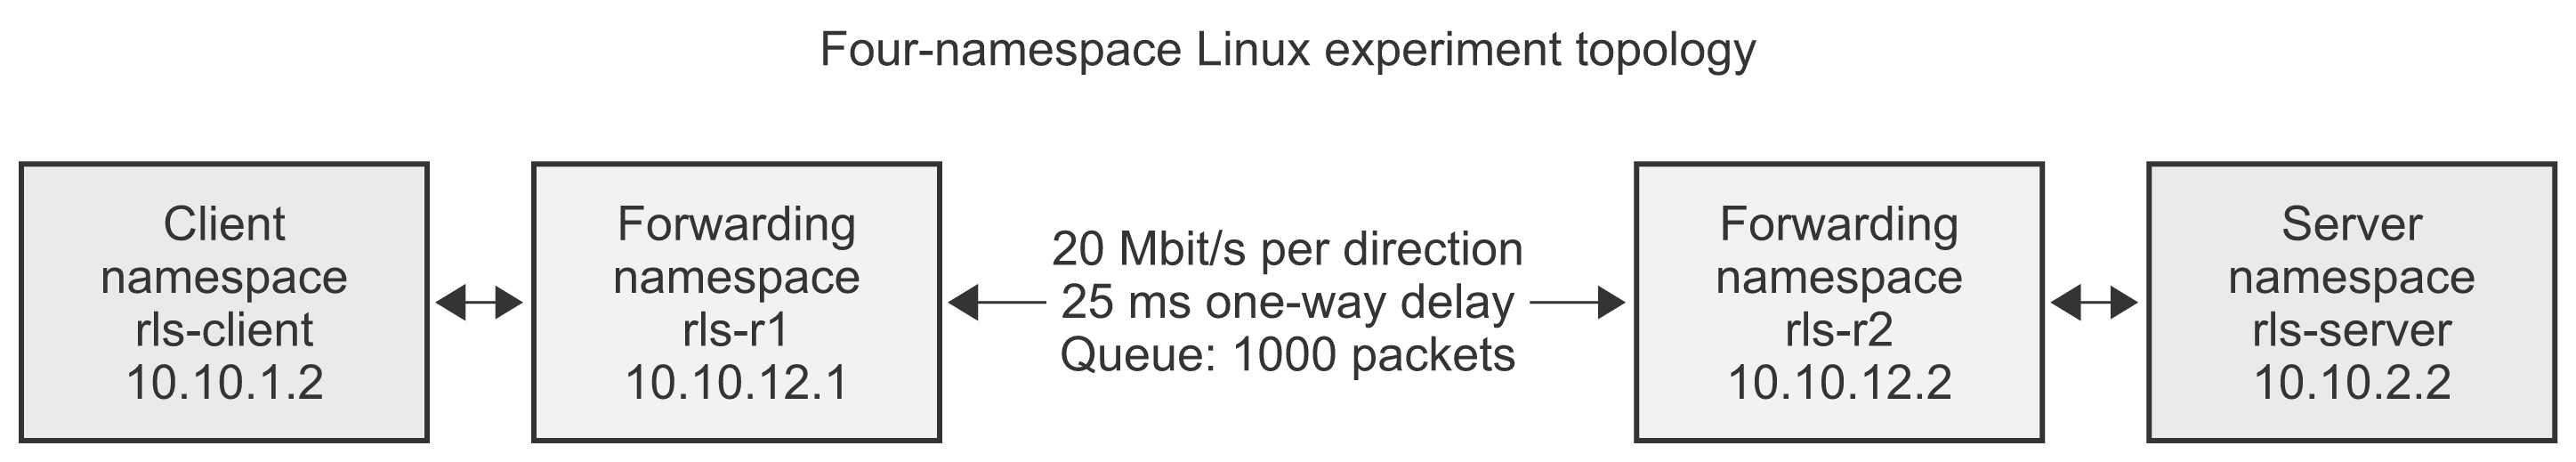
\includegraphics[width=\linewidth,height=0.48\textheight,keepaspectratio]{images/topology.png}
\captionof{figure}{Four-namespace Linux experimental topology. The server sends the measured payload to the client.}
\end{center}


The main topology has two endpoint namespaces and two forwarding namespaces. The core link carries 20 Mbit/s in each direction with 25 ms of one-way delay and a 1000-packet queue limit. The base round-trip time is approximately 50 ms. The supplementary dumbbell connects two client/server pairs across the same shaped link. Each supplementary run starts both transfers together \cite{ref12,ref13}.

\subsection*{3.4 Traceability and analysis}

Each run records the command, binary identity, configuration, performance data, and qlog traces. The source revision for the actual baseline binary is recorded in its \path{provenance.txt}. The sender qlog provides the window and flight-size samples. The server connection CSV supplies byte counts and connection times. The analysis weights each window sample by the time until the next sample. The comparison reports the means and sample variability across the three repetitions.

\label{sec:approach-end}

\clearpage
\section*{4. Implementation}
\label{sec:implementation}
\subsection*{4.1 Structural design and responsibilities}

\begin{center}
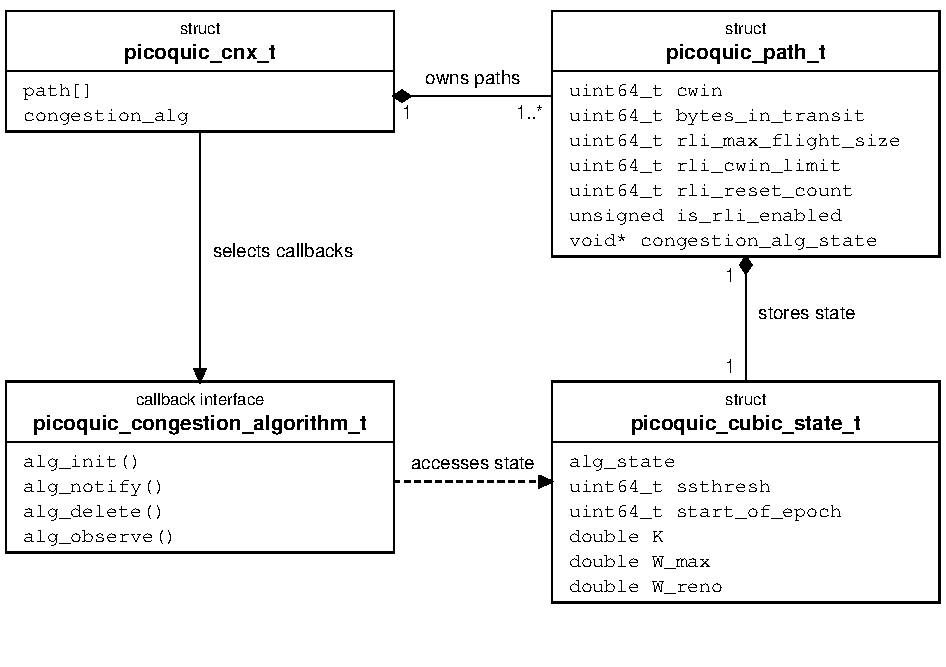
\includegraphics[width=\linewidth,height=0.48\textheight,keepaspectratio]{images/implementation-structure.pdf}
\captionof{figure}{Class-style structural diagram of the core C structs and callback interface. Selected fields are shown.}
\end{center}

picoquic\_cnx\_t holds path references and the selected congestion-control interface. A path holds cwnd, flight accounting, RLI fields, and an opaque pointer to its algorithm state. picoquic\_cubic\_state\_t remains the private CUBIC state. ACK information is passed through picoquic\_per\_ack\_state\_t to the notification callback. The diagram uses C struct and callback-interface stereotypes because the implementation is C; it does not invent C++ classes or member methods \cite{ref12}.


The sender module updates flight history where packet enqueue and dequeue accounting occurs. CUBIC computes limits, applies growth, and resets observation state during recovery. The logging modules export the resulting values. This distribution follows existing ownership: packet accounting remains in sender.c, policy remains in cubic.c, and diagnostics remain in the log writers and converters.


State is per path even though the live campaign selects one path. Focused tests create independent path instances to check isolation. That unit-level check does not establish correct live multipath behaviour, which would require dedicated connections and trace selection.


\subsection*{4.2 Initialization and packet accounting pseudocode}


\begingroup\footnotesize
\begin{verbatim}
ON_CUBIC_INITIALIZE(path, option):
    path.rli_enabled = option in {"rli", "rli=on", "on"}
    initialize_existing_CUBIC_state(path)
    path.cwnd = INITIAL_CWND
    path.maxFS = INITIAL_CWND if enabled else 0
    path.limit = 2 * INITIAL_CWND if enabled else 0
    path.reset_count = 0
    path.capped = false

ON_FLIGHTSIZE_UPDATE(path):
    if path.rli_enabled:
        path.maxFS = max(path.maxFS, path.bytes_in_transit)

ON_PACKET_ENQUEUE(path, packet_bytes):
    perform_existing_enqueue_and_flight_accounting()
    ON_FLIGHTSIZE_UPDATE(path)

ON_PACKET_DEQUEUE(path, packet):
    perform_existing_removal_and_flight_accounting()
    ON_FLIGHTSIZE_UPDATE(path)
\end{verbatim}
\endgroup

INITIAL\_CWND is 10 \(\times\) PICOQUIC\_MAX\_PACKET\_SIZE in this source, or 15,360 bytes in the recorded runs. Initializing maxFS to that value explains why a flight smaller than 15 KiB can still authorize growth toward 30 KiB in slow start. The maximum is not redefined as merely the largest small application frame. The source's send\_mtu is used for the additive congestion-avoidance limit.


\subsection*{4.3 Implementation map}

\begingroup\small\setlength{\tabcolsep}{4pt}\renewcommand{\arraystretch}{1.15}
\noindent\begin{tabular}{|>{\raggedright\arraybackslash}p{\dimexpr 0.33607\linewidth-2\tabcolsep-2\arrayrulewidth\relax}|>{\raggedright\arraybackslash}p{\dimexpr 0.66393\linewidth-2\tabcolsep-2\arrayrulewidth\relax}|}
\hline
\textbf{Source file / component} & \textbf{Implemented responsibility} \\ \hline
picoquic\_internal.h & Per-path RLI fields, flags, and reset counter. \\ \hline
sender.c & Maximum-flight accounting after enqueue and dequeue. \\ \hline
cubic.c & Activation, candidate growth, caps, epoch guard, recovery reset, and DCUBIC isolation. \\ \hline
logwriter.c; loglib/qlog*.c & Binary/direct qlog fields and optional-field conversion. \\ \hline
plot\_cwnd.py; experiments/*.py & Time-unit handling, trace parsing, graphs, validation, and campaign summaries. \\ \hline
\end{tabular}\endgroup
\par\vspace{0.6em}

Cap arithmetic saturates at UINT64\_MAX. Reset counting also saturates, avoiding wraparound in a long-running path. The Ubuntu verification did not separately exercise the overflow boundary.


\subsection*{4.4 Growth and reduction pseudocode}


\begingroup\footnotesize
\begin{verbatim}
ON_ACK_GROWTH(path, ack, phase):
    old = path.cwnd
    if not path.rli_enabled:
        run_existing_CUBIC_ACK_logic(); return
    candidate = existing_phase_candidate_with_RLI_growth(ack)
    limit = SAT_ADD(path.maxFS, path.send_mtu) if phase == CA
            else SAT_DOUBLE(path.maxFS)
    candidate = max(candidate, old)       # ACK cannot shrink cwnd
    path.capped = candidate > old and candidate > limit
    path.cwnd = max(old, min(candidate, limit))
    path.W_reno = min(path.W_reno, path.cwnd)
    path.limit = limit

ON_REAL_WINDOW_REDUCTION(path, congestion_event):
    run_existing_CUBIC_recovery_response(congestion_event)
    if path.rli_enabled:
        path.maxFS = 0; path.limit = 0; path.capped = false
        path.reset_count = SAT_ADD(path.reset_count, 1)
\end{verbatim}
\endgroup

The pseudocode summarizes the RLI logic and does not replace the existing ACK, recovery, or RTT state machine. The first live pilot exposed an ACK-driven decrease after an epoch adjustment. The corrected helper preserves the old window in that path. Genuine reductions still use recovery and clear maxFS. Spurious recovery may restore CUBIC window and epoch state, but does not restore the pre-reduction flight maximum \cite{ref12}.


\subsection*{4.5 Verification and instrumentation}

qlog exports rli\_max\_flight\_size, rli\_cwnd\_limit, rli\_capped, and rli\_reset\_count. The counter makes a reset observable when the flight has already rebuilt before the next snapshot. The trace validator rejects unreset decreases, uncapped growth, missing cap exercise, and maximum-flight values below observed flight. A retained peak above both adjacent samples is accepted as a possible intermediate event and counted, rather than incorrectly rejected.


\begingroup\small\setlength{\tabcolsep}{4pt}\renewcommand{\arraystretch}{1.15}
\noindent\begin{tabular}{|>{\raggedright\arraybackslash}p{\dimexpr 0.27049\linewidth-2\tabcolsep-2\arrayrulewidth\relax}|>{\raggedright\arraybackslash}p{\dimexpr 0.72951\linewidth-2\tabcolsep-2\arrayrulewidth\relax}|}
\hline
\textbf{Saved verification} & \textbf{Outcome and scope} \\ \hline
Full regression & Both registered CTest entries passed for both versions. The baseline ran 667 internal checks and the RLI build ran 668. \\ \hline
Focused C checks & The \texttt{cubic\_rli} test covered growth caps, packet accounting, loss, ECN, timeout, spurious recovery, and CUBIC epoch handling. \\ \hline
Live trace checks & All twelve RLI connections passed the applicable observed-invariant checks. \\ \hline
\end{tabular}\endgroup
\par\vspace{0.6em}

\label{sec:implementation-end}

\clearpage
\section*{5. Result and Analysis}
\label{sec:results}
\subsection*{5.1 Experimental parameters}

The campaign ran on 10 November 2026, on Ubuntu 26.04 LTS with kernel \texttt{7.0.0-42-generic}. GCC 15.2.0 and CMake 4.2.3 built both revisions \cite{ref13}.
Each access link has 1000 Mbit/s bandwidth and 5 ms delay in each direction.
The core link has 20 Mbit/s bandwidth and 25 ms delay in each direction.
Each shaped interface has a 1000-packet queue limit.
The nominal base RTT is 70 ms; the corresponding bandwidth-delay product is about 171 KiB.
Ping and qdisc checks verified both endpoint pairs.

Single-flow throughput uses the server's application bytes and connection duration.
Window and flight-size samples come from sender qlogs; final RTT comes from the server performance CSV.
Detailed graphs show repetition one. Tables use all three repetitions per mode.
The previous campaign is retained in a local backup, separate from these measurements.
\begin{center}
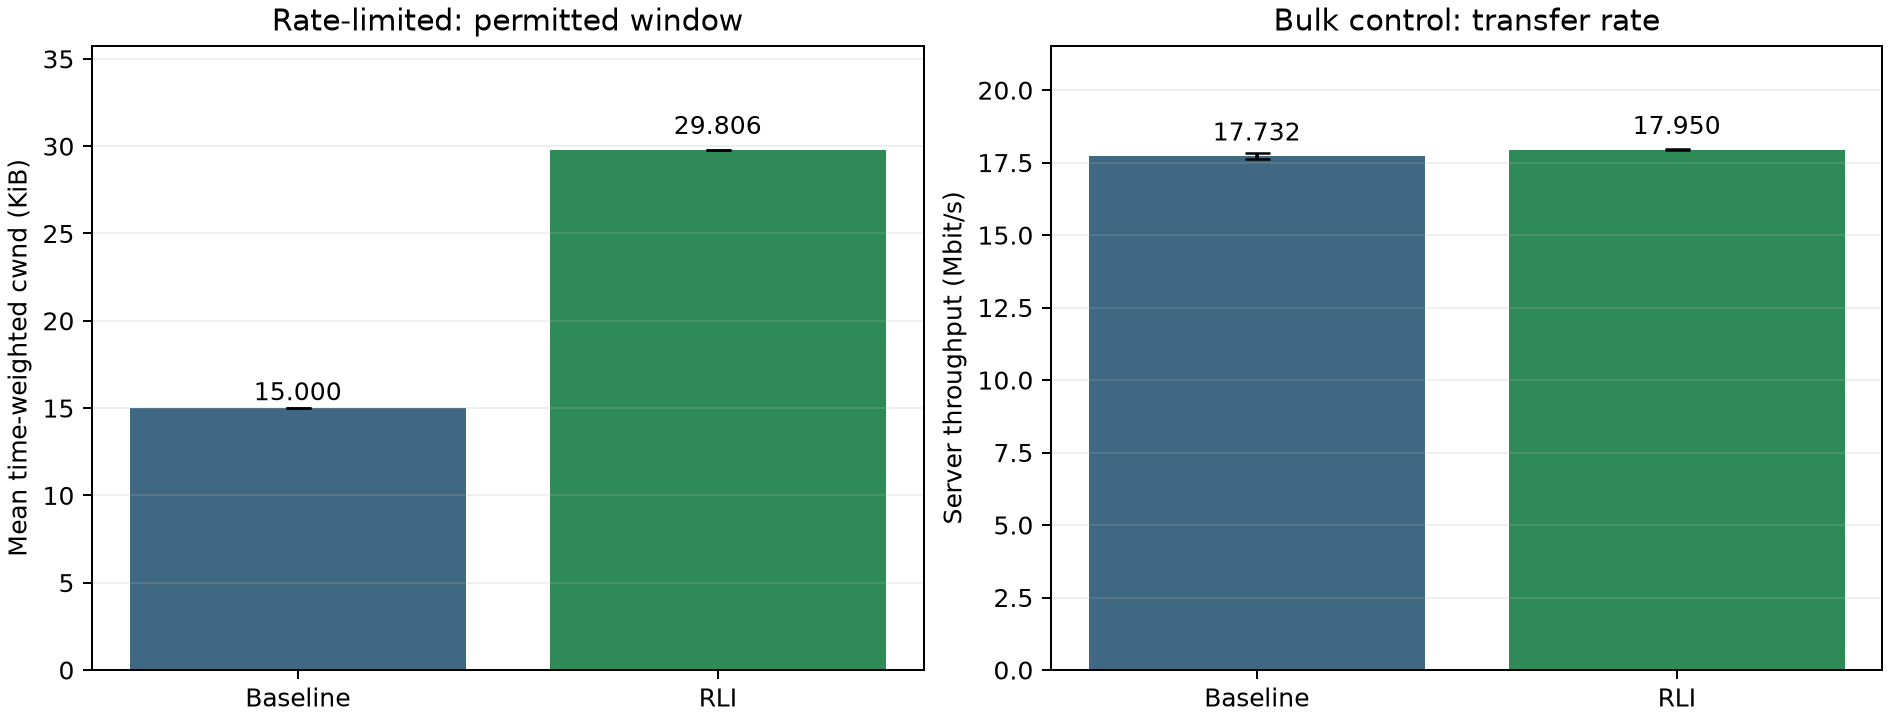
\includegraphics[width=\linewidth,height=.32\textheight,keepaspectratio]{images/native-overview.png}
\captionof{figure}{Fresh three-run means with sample standard-deviation bars for fixed-rate cwnd and bulk throughput.}
\end{center}

\subsection*{5.2 Fixed-rate workload}
\begin{center}\small\begin{tabular}{lrrrr}
Mode & Rate (Mbit/s) & Final cwnd (KiB) & Mean cwnd (KiB) & Final RTT (ms) \\ \hline
Original & 0.189391 & 15.00 & 15.00 & 71.794 \\
RLI & 0.189369 & 30.00 & 29.83 & 71.817 \\
\end{tabular}\end{center}

Each transfer delivers 480,000 bytes at an offered rate of approximately 192 kbit/s.
The largest observed RLI flight is 3426 bytes. The initialized 15 KiB maxFS sets the 30 KiB slow-start ceiling.
A larger permitted window does not increase the application's supply of data.
The experiment does not measure the completion time of a later burst.
\begin{center}
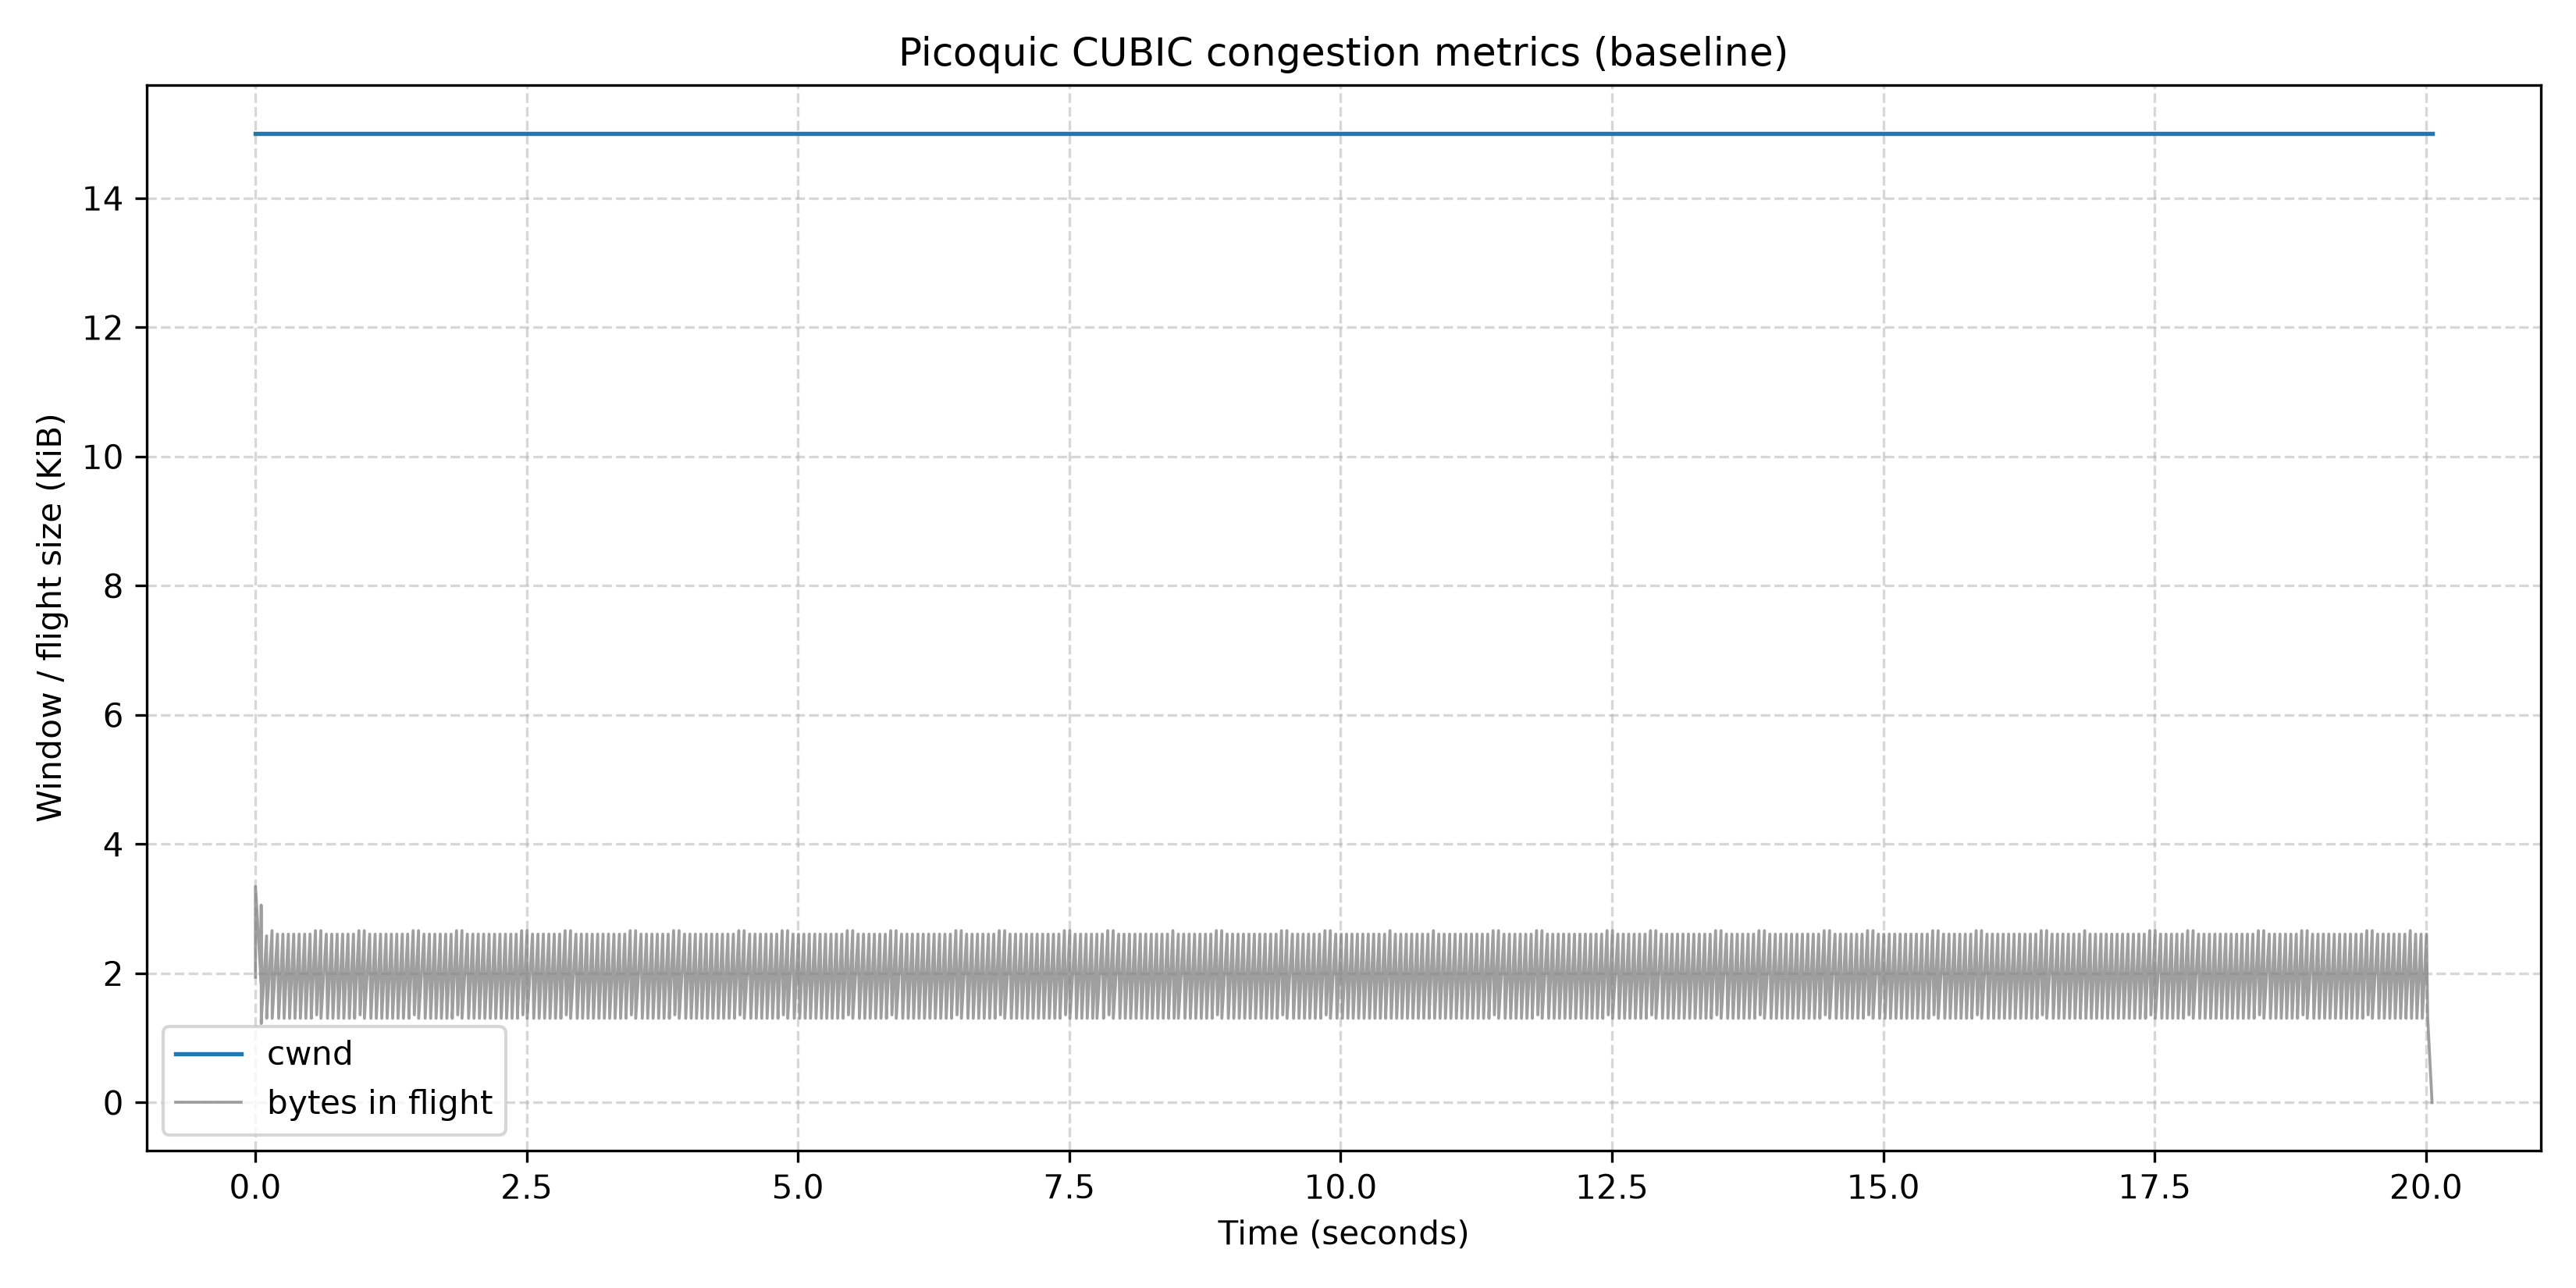
\includegraphics[width=\linewidth,height=.25\textheight,keepaspectratio]{images/native-rate-limited-baseline-1.png}
\captionof{figure}{Original CUBIC, fresh fixed-rate repetition one.}
\end{center}
\begin{center}
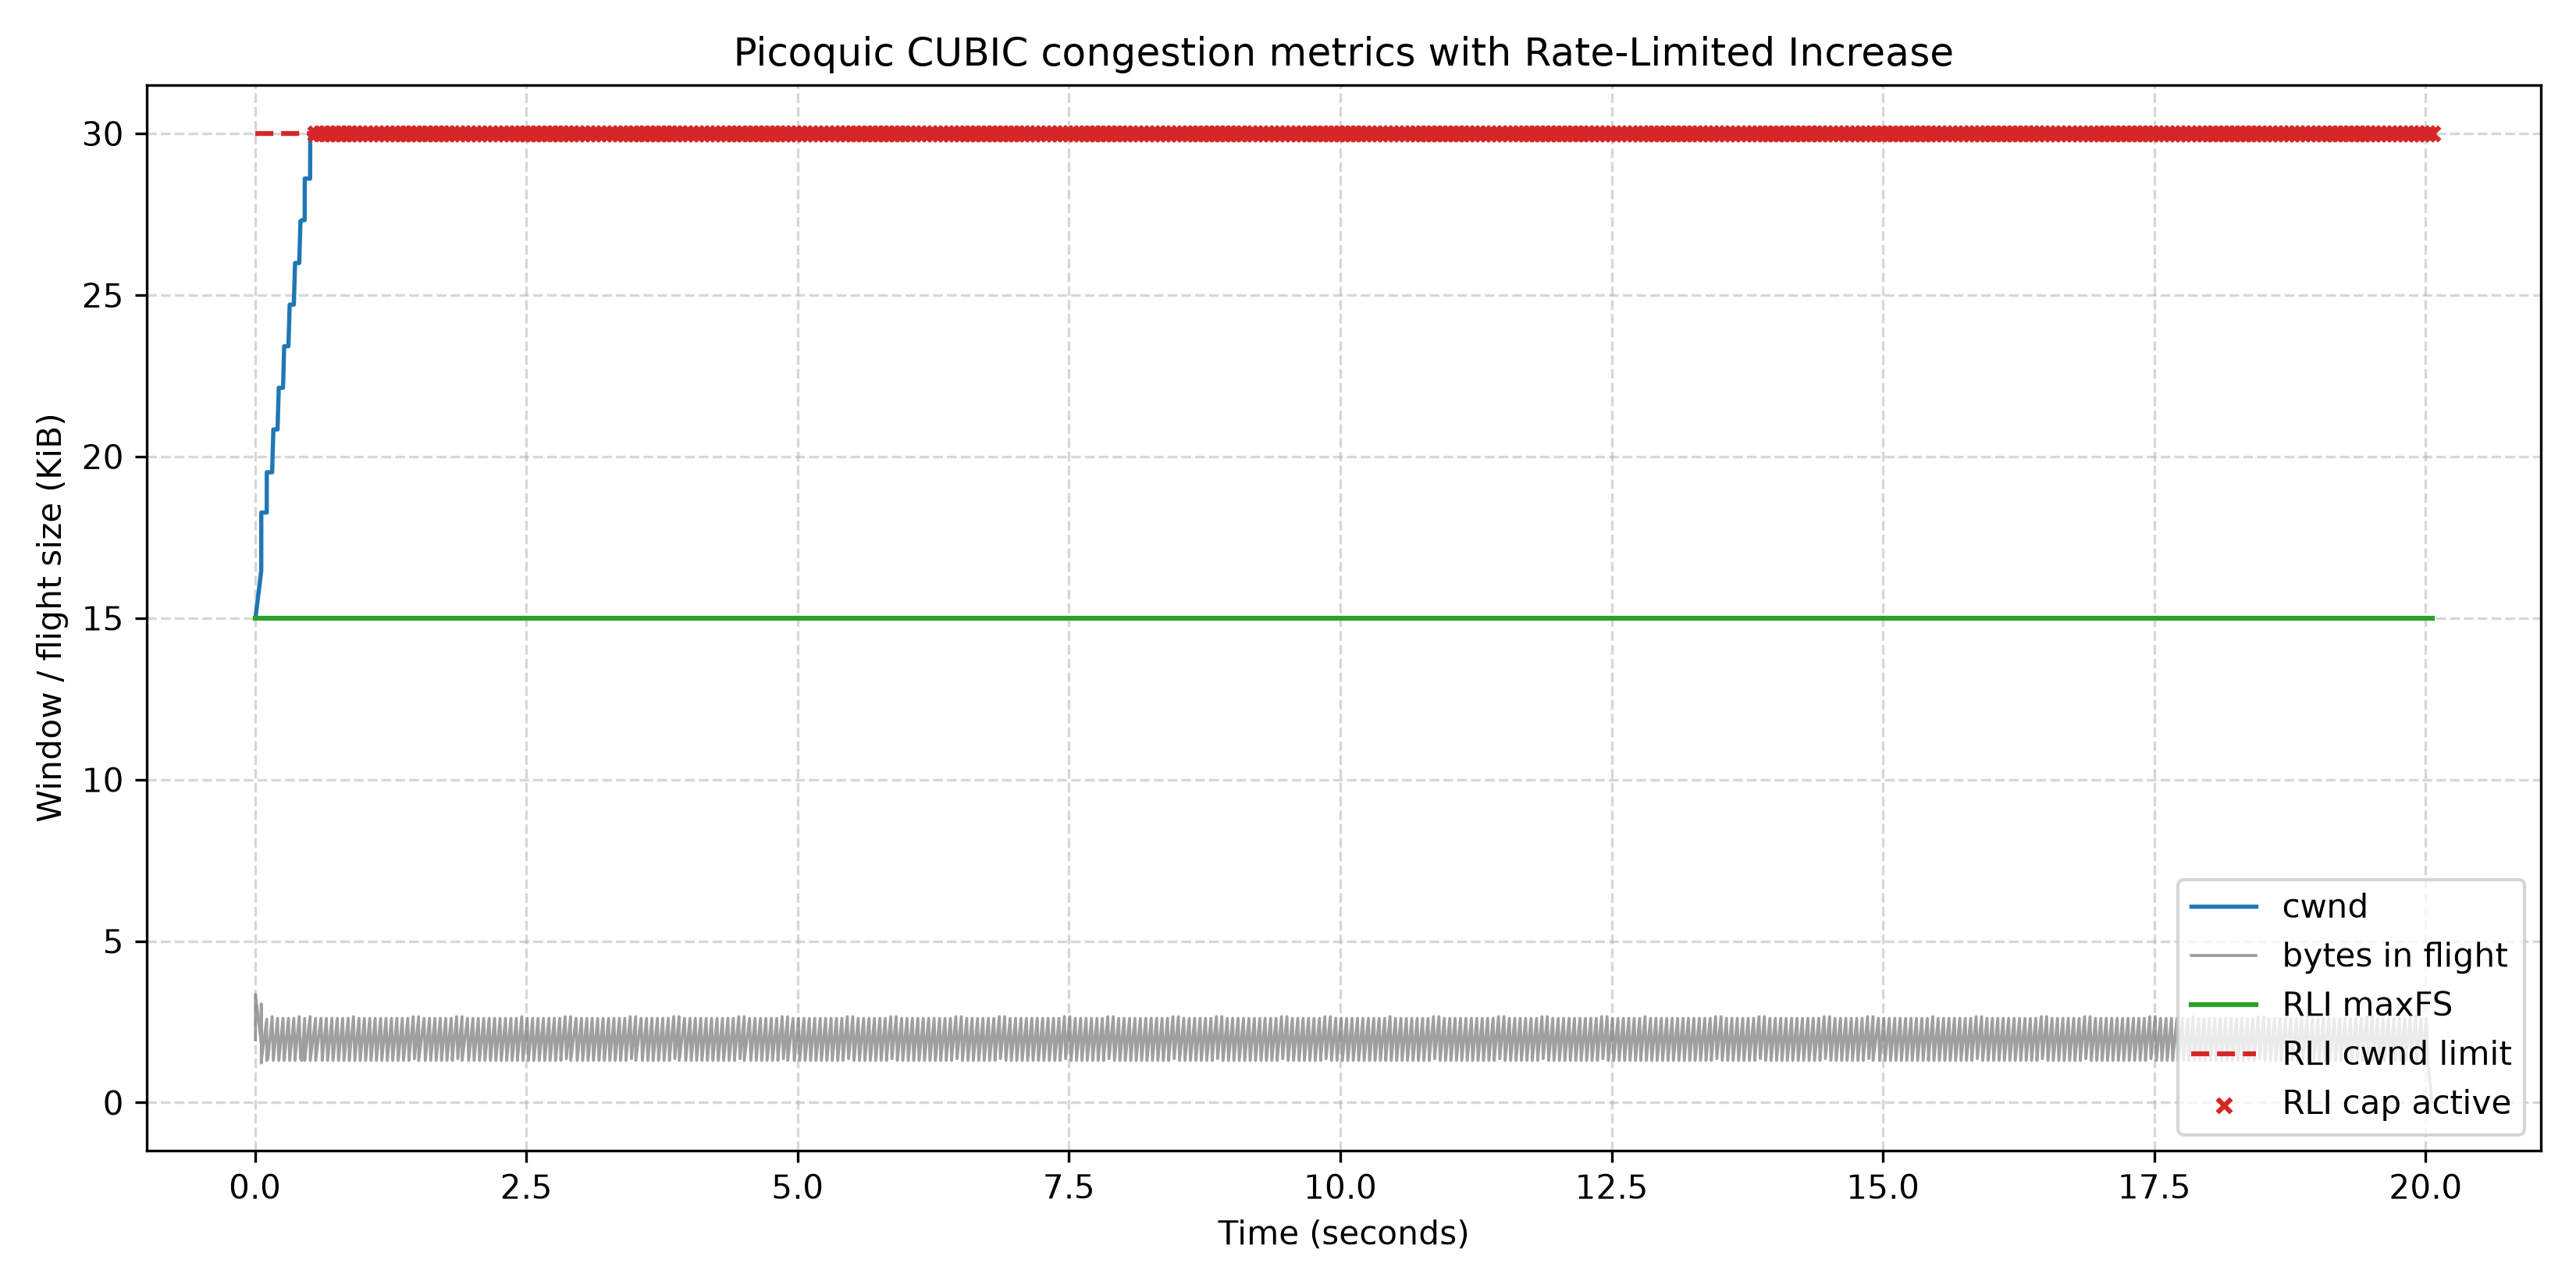
\includegraphics[width=\linewidth,height=.25\textheight,keepaspectratio]{images/native-rate-limited-rli-1.png}
\captionof{figure}{CUBIC with RLI, fresh fixed-rate repetition one.}
\end{center}

\subsection*{5.3 Single-flow bulk transfers}
\begin{center}\small\begin{tabular}{lrrrr}
Mode & Rate (Mbit/s) & Final cwnd (KiB) & Mean cwnd (KiB) & Final RTT (ms) \\ \hline
Original & 17.096857 & 554.94 & 504.39 & 211.599 \\
RLI & 17.602599 & 358.20 & 286.78 & 139.168 \\
\end{tabular}\end{center}

The observed mean throughput change is +2.96\%.
Paired RLI-minus-baseline differences are +0.449, +0.232, +0.836 Mbit/s.
Three repetitions describe this configuration; they do not establish a general performance gain or regression.
Final smoothed RTT is an endpoint statistic, not a direct queue-occupancy measurement.
The twelve single-flow runs record 0 retransmissions in total.
\begin{center}
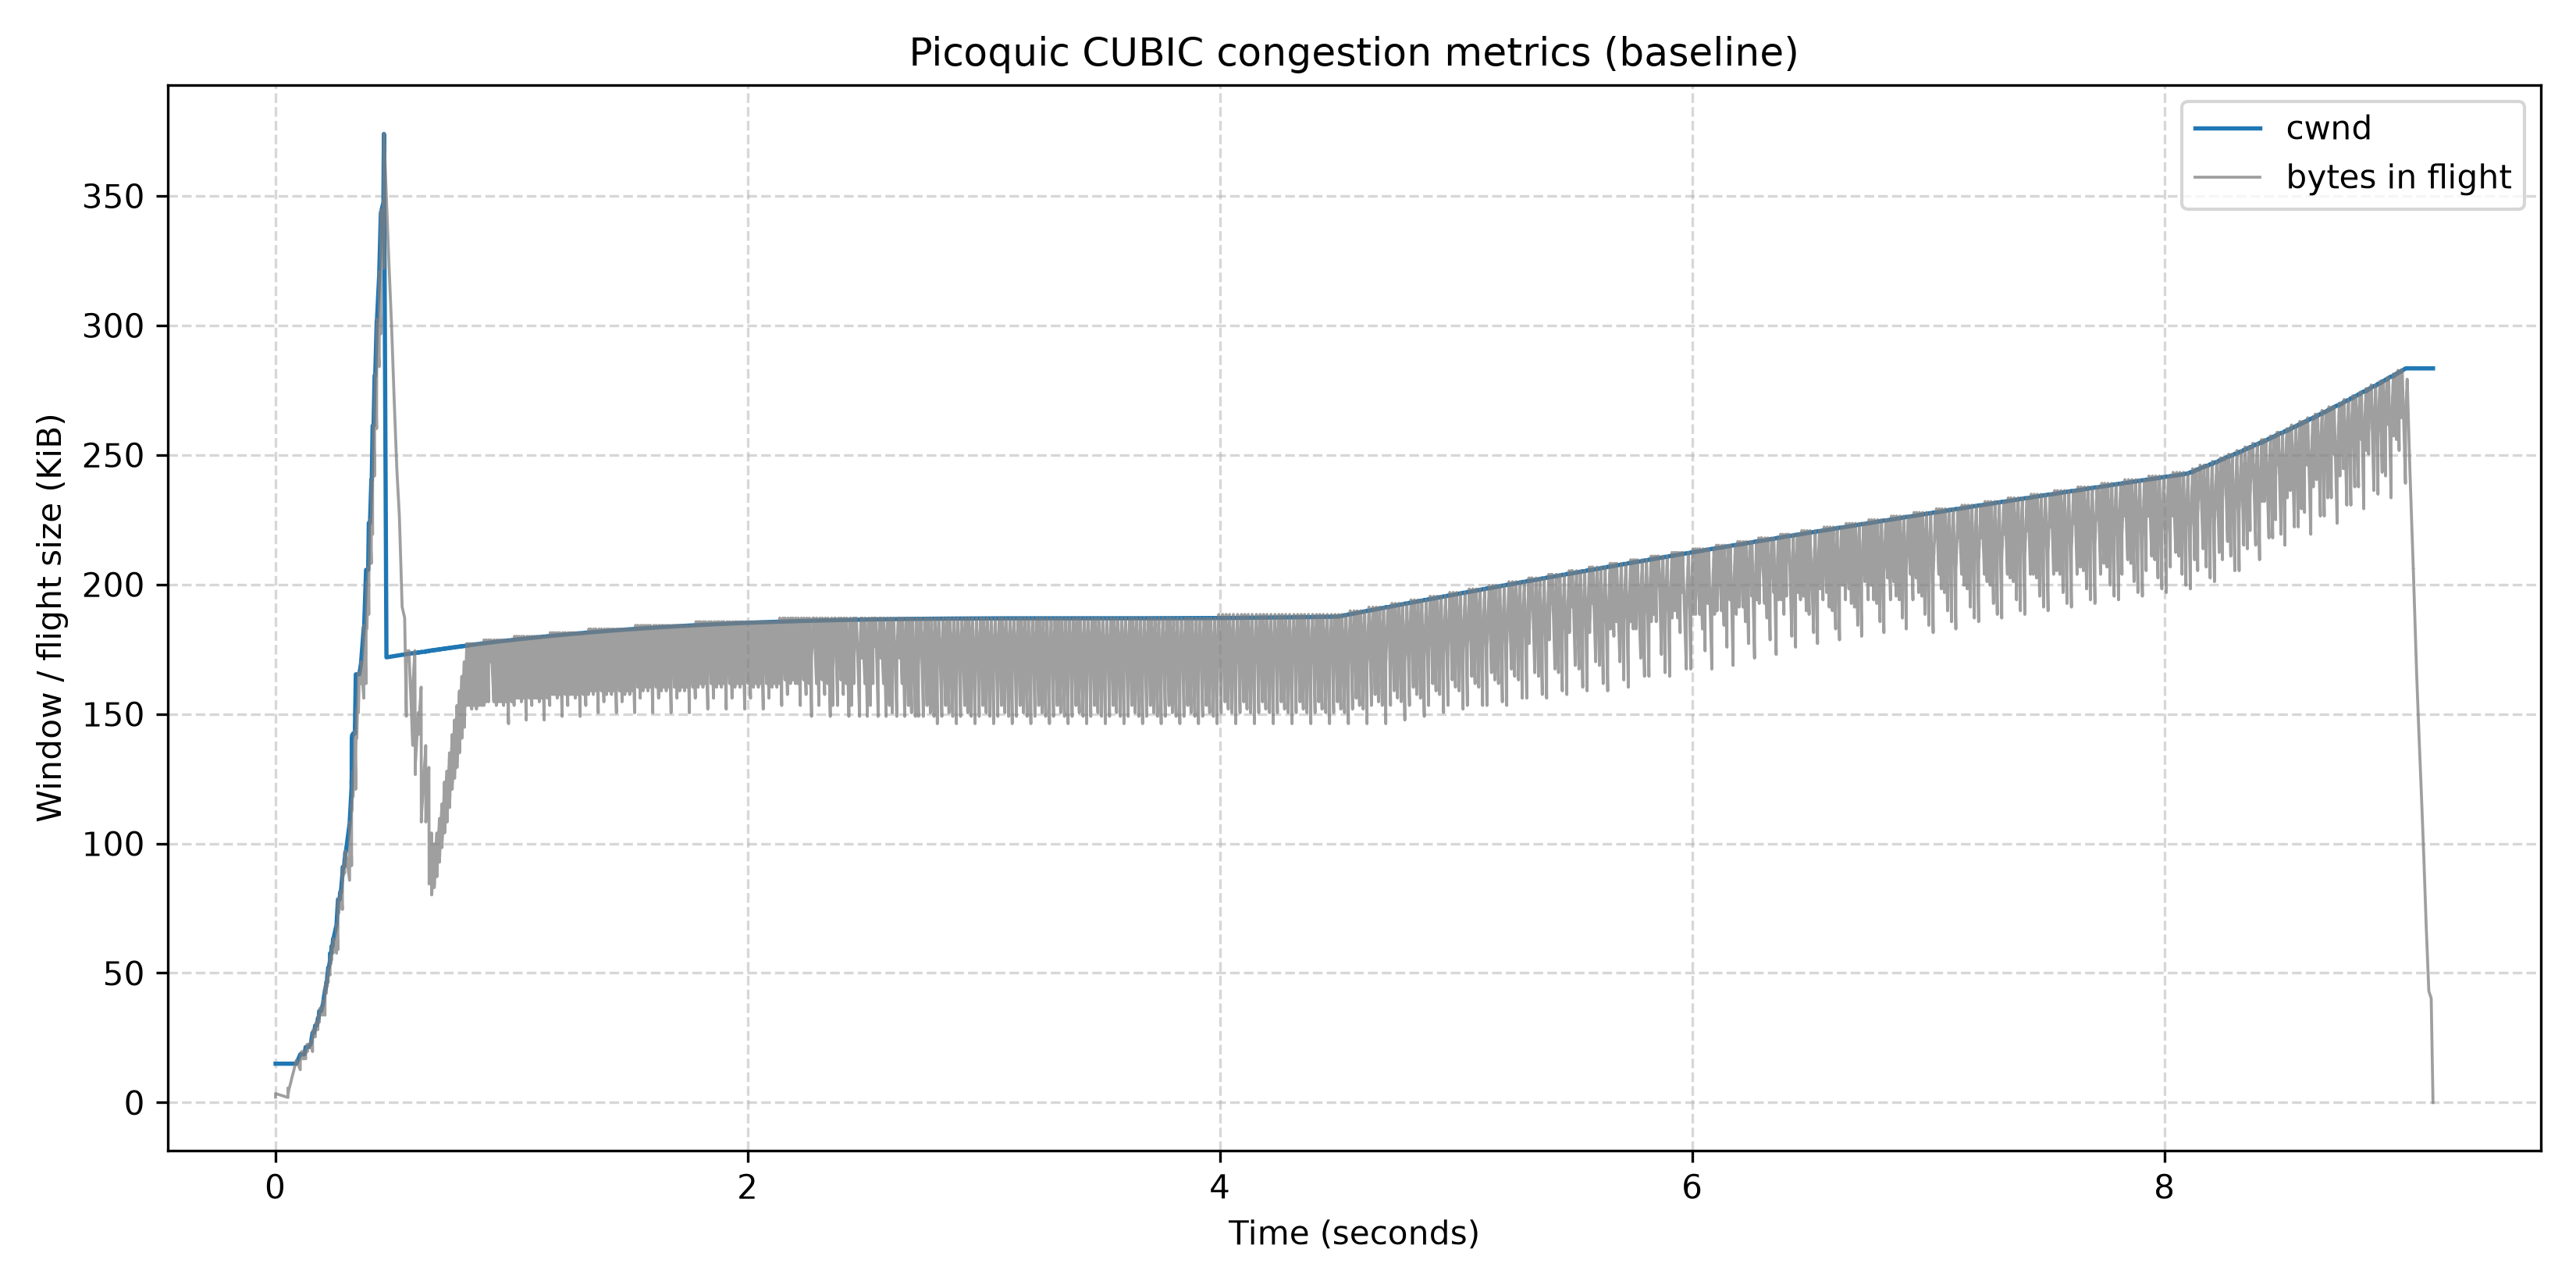
\includegraphics[width=\linewidth,height=.25\textheight,keepaspectratio]{images/native-bulk-baseline-1.png}
\captionof{figure}{Original CUBIC, fresh bulk repetition one.}
\end{center}
\begin{center}
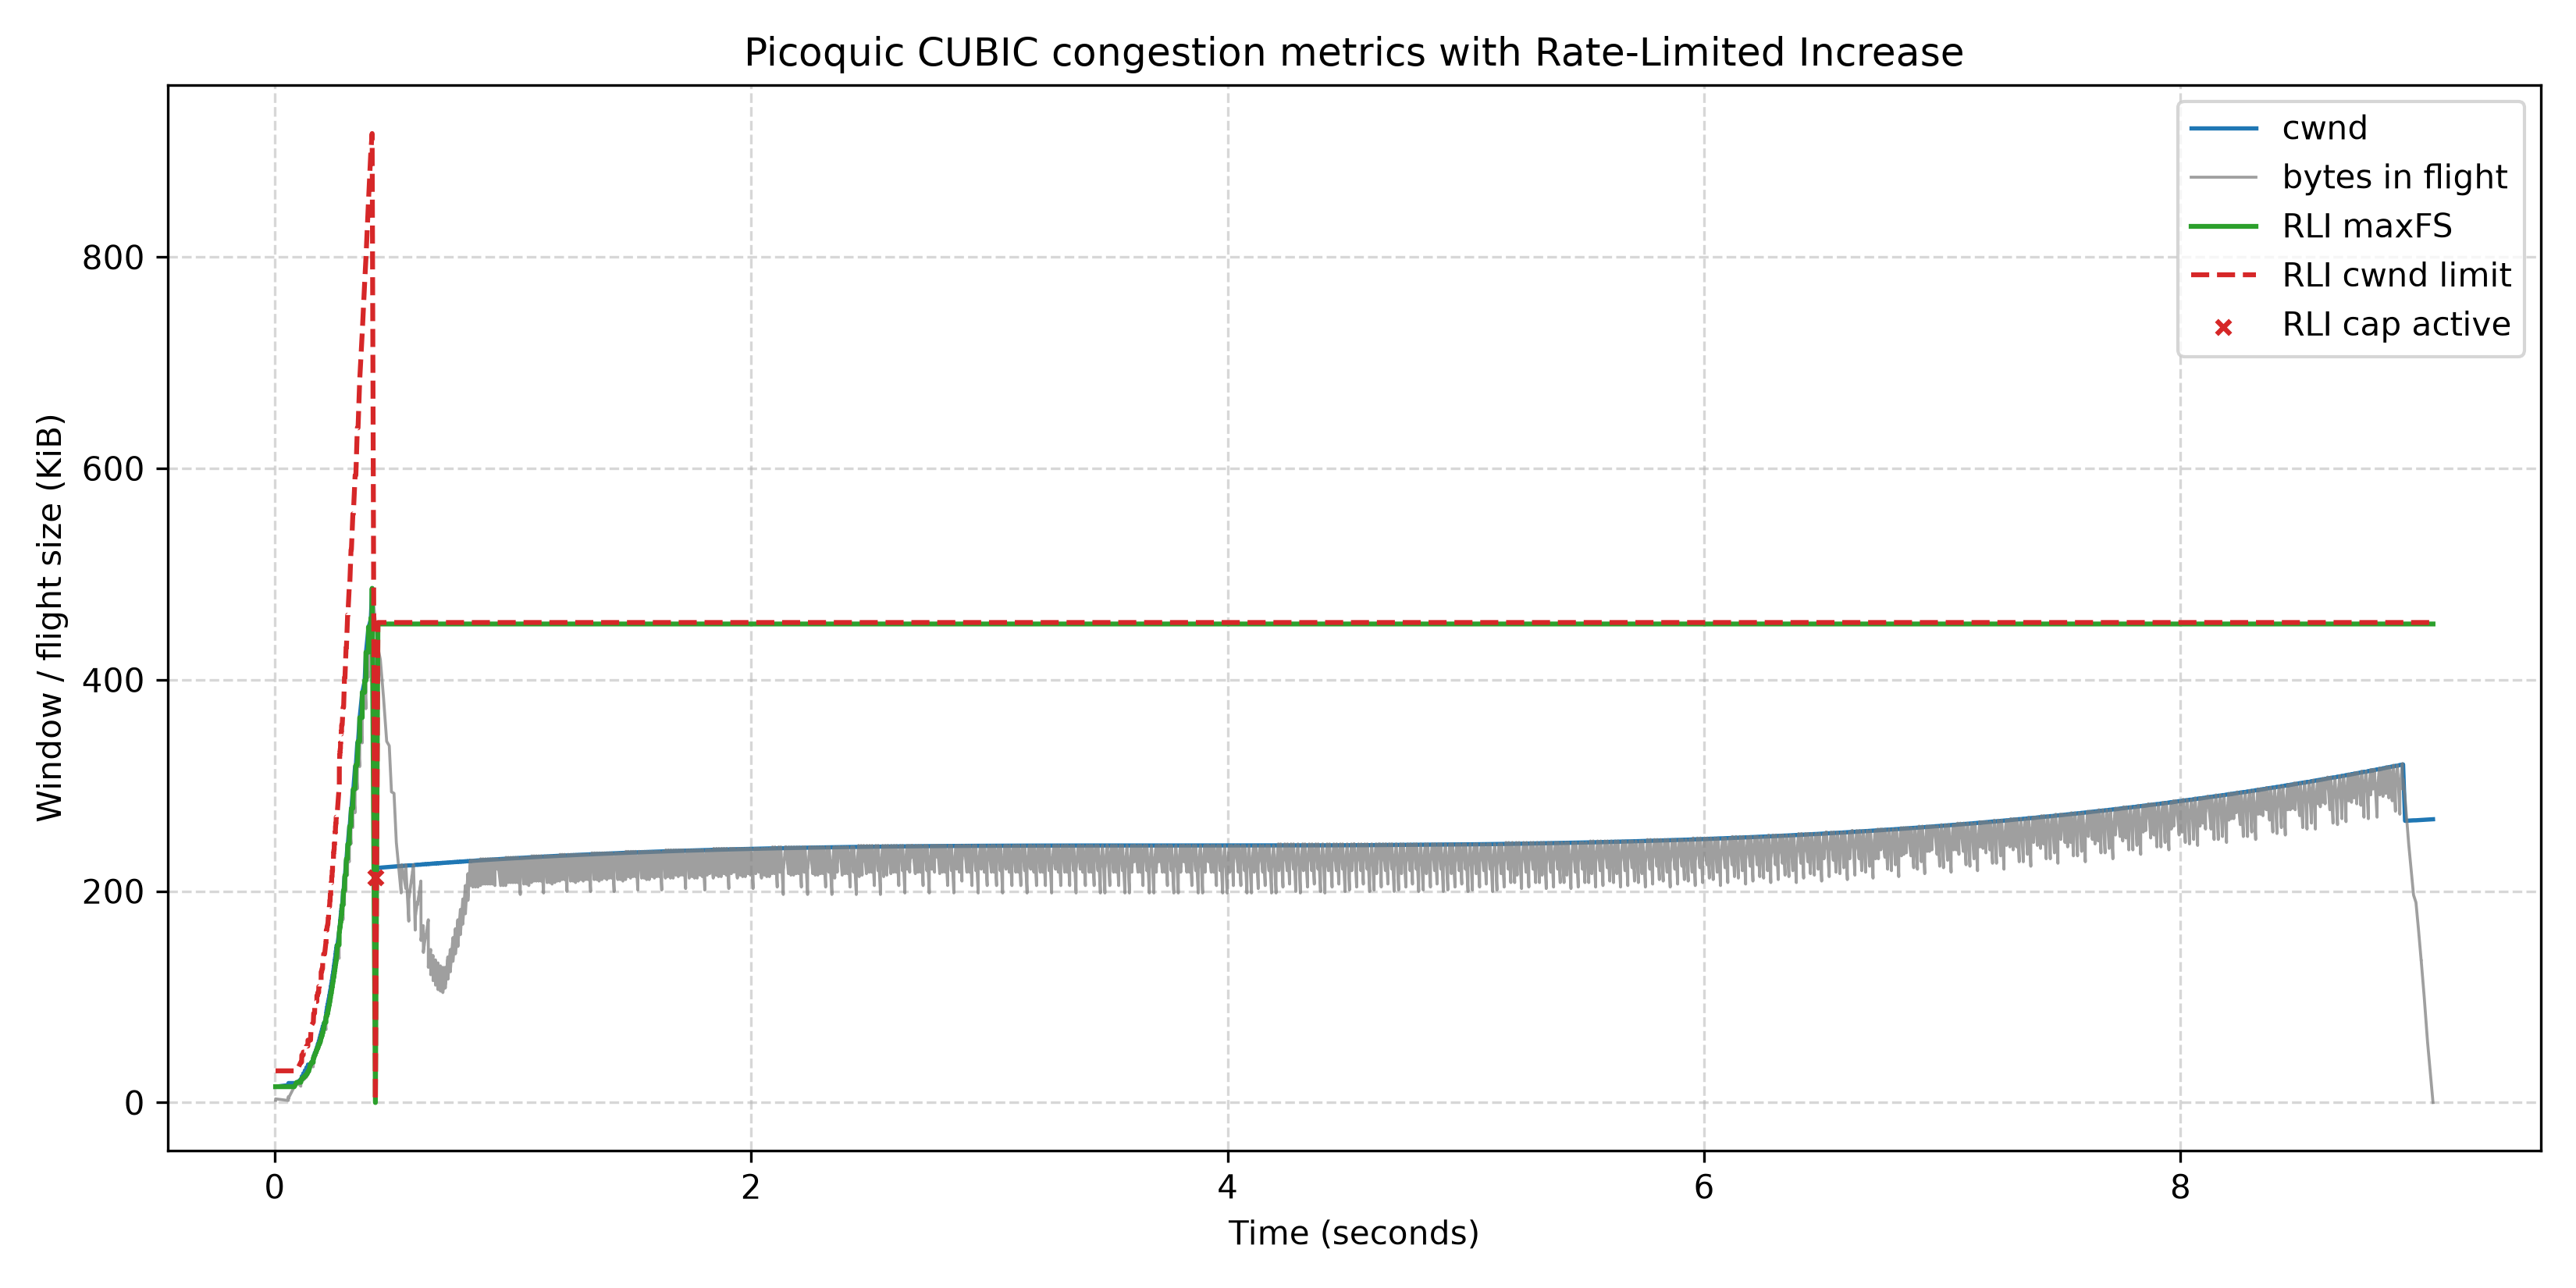
\includegraphics[width=\linewidth,height=.25\textheight,keepaspectratio]{images/native-bulk-rli-1.png}
\captionof{figure}{CUBIC with RLI, fresh bulk repetition one.}
\end{center}

\subsection*{5.4 Two flows sharing the dumbbell}
\begin{center}\small\begin{tabular}{lrrr}
Mode & Combined Mbit/s & Jain index & Mean retransmissions \\ \hline
Original & 18.596 & 0.98700 & 190.3 \\
RLI & 18.580 & 0.98910 & 0.0 \\
\end{tabular}\end{center}

Combined throughput uses the interval from client launch until both clients exit.
Each flow's connection rate uses its server's own connection interval.
The Jain index uses those two per-connection rates; it does not measure instantaneous fairness.
Both connections use the same algorithm in each experiment.
The mean combined-throughput change is -0.08\%.
\begin{center}
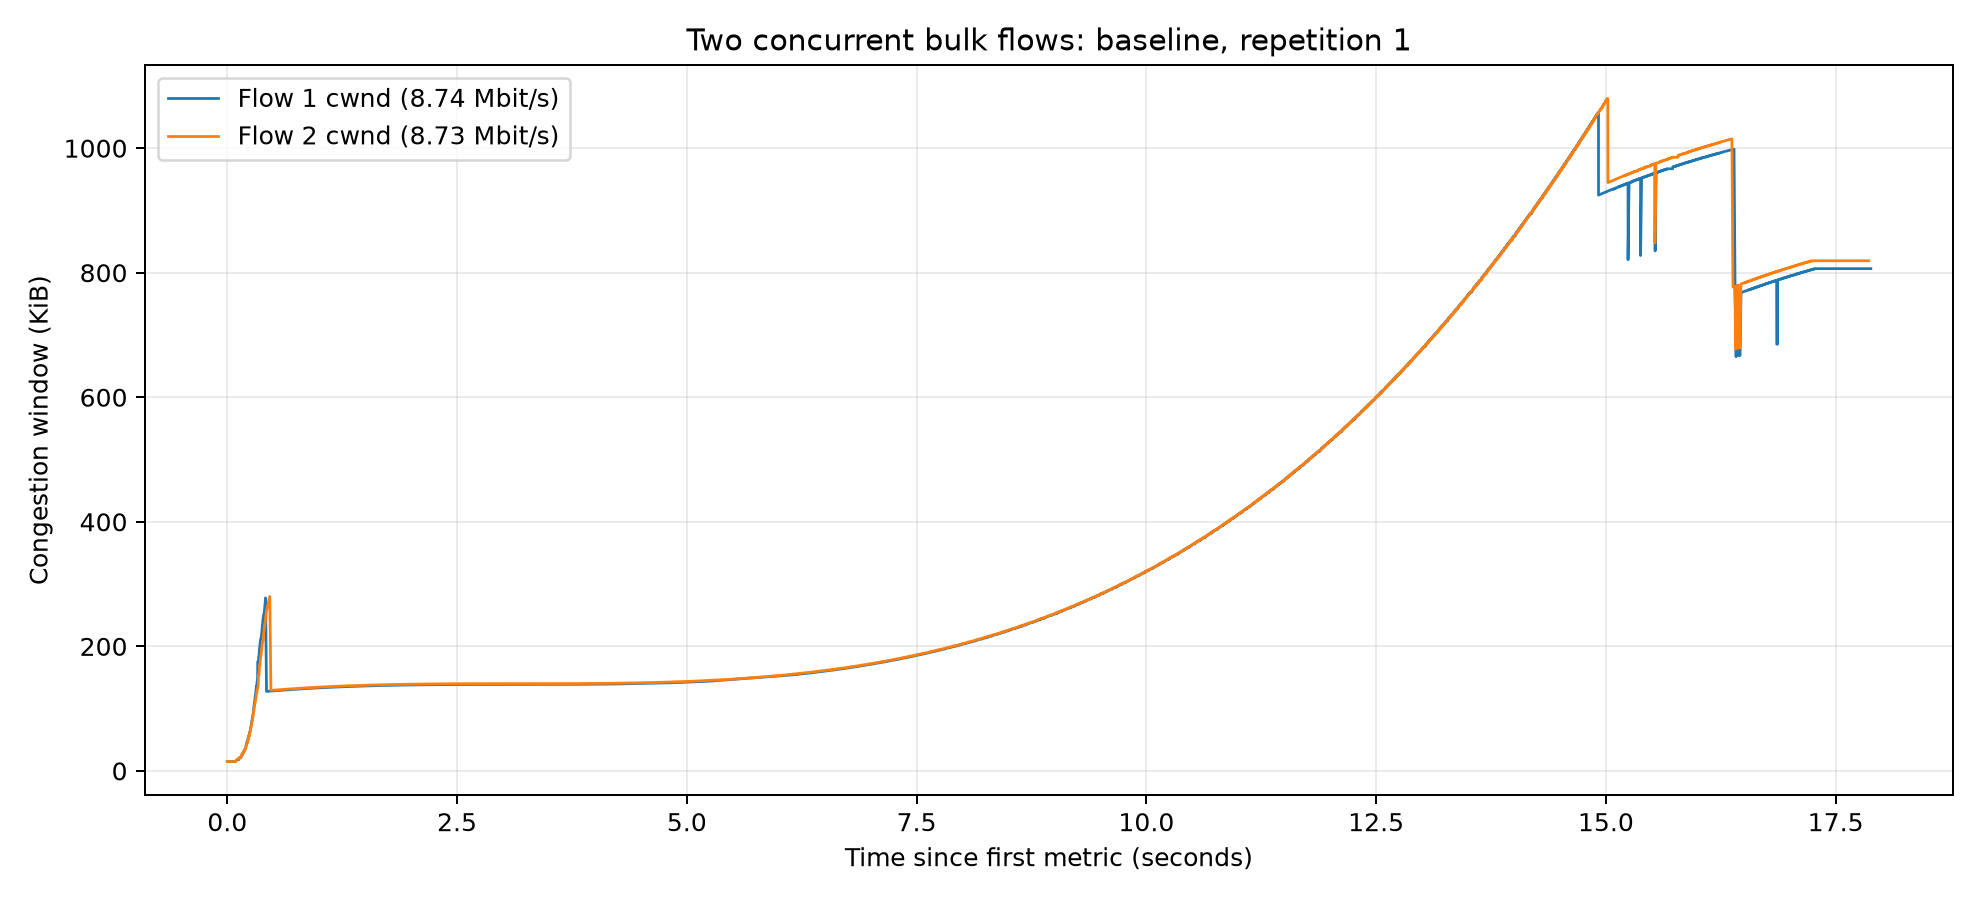
\includegraphics[width=\linewidth,height=.25\textheight,keepaspectratio]{images/native-dumbbell-baseline-1.png}
\captionof{figure}{Two competing flows with original CUBIC, fresh repetition one.}
\end{center}
\begin{center}
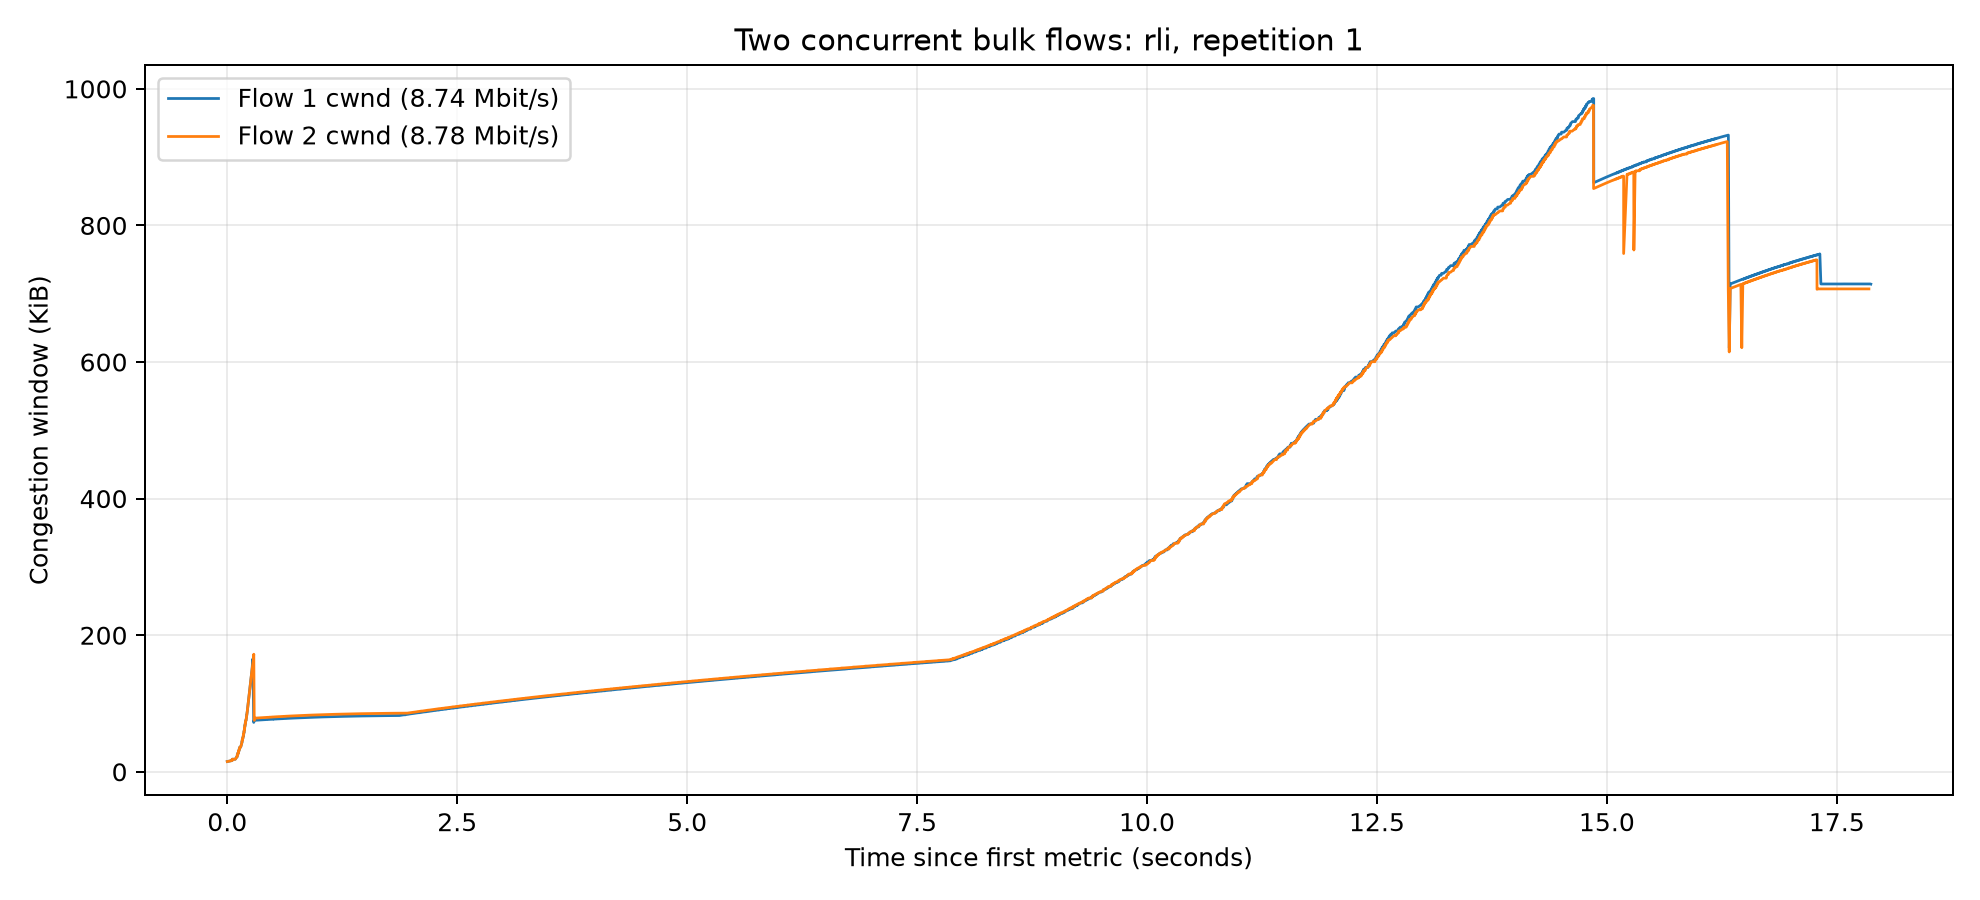
\includegraphics[width=\linewidth,height=.25\textheight,keepaspectratio]{images/native-dumbbell-rli-1.png}
\captionof{figure}{Two competing flows with RLI, fresh repetition one.}
\end{center}

\subsection*{5.5 Validation and comparison}

The current trace validator passes all six single-flow RLI traces and all six competing RLI connections.
Fixed-rate cases require an active cap. RLI bulk cases additionally require a window reduction and an observable flight-history reset.
Both builds pass their registered CTest suites. The separate cubic\_rli test also passes.
Reset counters make history resets observable even when flight size rebuilds between snapshots.

\begin{center}\small
\begin{tabularx}{\linewidth}{@{}p{0.25\linewidth}XX@{}}
\textbf{Aspect} & \textbf{Reference behavior} & \textbf{Observed result}\\ \hline
Application limitation & RFC 9438 suppresses growth in application-limited intervals \cite{ref2}. & RLI grows cwnd from 15 to 30 KiB at the slow-start cap.\\[3pt]
Growth bound & The RLI draft bounds increases using flight history \cite{ref1}. & Fixed-rate runs exercise the slow-start cap. The focused test checks the selected congestion-avoidance cap.\\[3pt]
Window retention & RFC 7661 considers windows that have not been exercised \cite{ref6}. & These experiments evaluate bounded growth, not window aging.\\
\end{tabularx}
\end{center}
\label{sec:results-end}


\clearpage
\section*{6. Conclusions and Future Work}
\label{sec:conclusions}

This project implements bounded growth for a rate-limited CUBIC sender in picoquic. The sender tracks the maximum flight size per path and clears that history when the congestion window falls. Both builds passed their registered regression suites.

The Ubuntu experiments show that RLI raises the fixed-rate congestion window from 15 to 30 KiB, as expected from the slow-start rule. The two versions deliver the same amount of data at about 0.189 Mbit/s. Bulk and competing-flow measurements describe behavior when the application supplies more data. All twelve RLI connections pass the applicable trace checks.

A later experiment should bring the sender into congestion avoidance, reduce the offered rate, and then release a burst. This would test the congestion-avoidance cap in a live limited transfer and measure burst completion time. Controlled loss and tests with different competing algorithms would extend the recovery and fairness evaluation.
\label{sec:conclusions-end}

\clearpage
\phantomsection\label{sec:references}
\begingroup\small
\begin{thebibliography}{99}
\bibitem{ref1} M. Welzl, T. Henderson, G. Fairhurst, and M. P. Tahiliani. Increase of the Congestion Window when the Sender Is Rate-Limited. Internet-Draft, \nolinkurl{draft-ietf-ccwg-ratelimited-increase-11}, 6 September 2026. Sections 3 and 4.5. \url{https://www.ietf.org/archive/id/draft-ietf-ccwg-ratelimited-increase-11.html}
\bibitem{ref2} L. Xu, S. Ha, I. Rhee, V. Goel, and L. Eggert. CUBIC for Fast and Long-Distance Networks. RFC 9438, August 2023. Sections 4.2 and 5.8. \url{https://www.rfc-editor.org/rfc/rfc9438.html}
\bibitem{ref3} J. Iyengar and I. Swett. QUIC Loss Detection and Congestion Control. RFC 9002, May 2021. Section 7.8. \url{https://www.rfc-editor.org/rfc/rfc9002.html}
\bibitem{ref4} J. Iyengar and M. Thomson. QUIC: A UDP-Based Multiplexed and Secure Transport. RFC 9000, May 2021. \url{https://www.rfc-editor.org/rfc/rfc9000.html}
\bibitem{ref5} M. Allman, V. Paxson, and E. Blanton. TCP Congestion Control. RFC 5681, September 2009. \url{https://www.rfc-editor.org/rfc/rfc5681.html}
\bibitem{ref6} G. Fairhurst, A. Sathiaseelan, and R. Secchi. Updating TCP to Support Rate-Limited Traffic. RFC 7661, October 2015. Experimental. \url{https://www.rfc-editor.org/rfc/rfc7661.html}
\bibitem{ref7} P. Balasubramanian, Y. Huang, and M. Olson. HyStart++: Modified Slow Start for TCP. RFC 9406, May 2023. \url{https://www.rfc-editor.org/rfc/rfc9406.html}
\bibitem{ref8} Private Octopus. picoquic: official source repository. The local experiment revisions are identified separately in Appendix A. \url{https://github.com/private-octopus/picoquic}
\bibitem{ref9} Linux man-pages project. network\_namespaces(7): overview of Linux network namespaces. \url{https://man7.org/linux/man-pages/man7/network_namespaces.7.html}
\bibitem{ref10} iproute2 manual. tc-netem(8): Network Emulator. \url{https://man7.org/linux/man-pages/man8/tc-netem.8.html}
\bibitem{ref12} Local project sources and implementation records: picoquic/cubic.c, sender.c, picoquic\_internal.h; picoquictest/congestion\_test.c; PROJECT\_PROGRESS.md, IMPLEMENTATION\_PLAN.md, and results/README.md; topology/setup.sh; experiments/collect\_results.py and validate\_rli.py.
\bibitem{ref13} OSNT Project. Ubuntu network-namespace campaign, 10 November 2026. The local \path{results/} bundle contains source identifiers, binary hashes, measurements, figures, and raw qlogs. The previous campaign is retained separately. \url{https://github.com/yoman12357/OSNT_Project}
\end{thebibliography}
\endgroup


\clearpage
\section*{Appendix A. Run records}
\label{sec:appendix}
\begin{center}\small\begin{tabular}{lrrrrr}
Workload & Mode & Run & Mbit/s & Duration (s) & Final cwnd (KiB) \\ \hline
rate-limited & baseline & 1 & 0.190202 & 20.189041 & 15.00 \\
rate-limited & rli & 1 & 0.190171 & 20.192343 & 30.00 \\
rate-limited & baseline & 2 & 0.190196 & 20.189743 & 15.00 \\
rate-limited & rli & 2 & 0.190194 & 20.189867 & 30.00 \\
rate-limited & baseline & 3 & 0.19014 & 20.195616 & 15.00 \\
rate-limited & rli & 3 & 0.190192 & 20.19008 & 30.00 \\
bulk & baseline & 1 & 17.731435 & 9.461879 & 283.41 \\
bulk & rli & 1 & 17.939509 & 9.352134 & 268.04 \\
bulk & baseline & 2 & 17.823301 & 9.41311 & 304.68 \\
bulk & rli & 2 & 17.957932 & 9.34254 & 261.98 \\
bulk & baseline & 3 & 17.640233 & 9.510798 & 295.67 \\
bulk & rli & 3 & 17.951898 & 9.34568 & 264.75 \\
\end{tabular}\end{center}

\subsection*{A.1 Source and trace records}

The original build uses commit \texttt{5a4eba47}. The RLI build uses commit \texttt{60323926}. The Ubuntu archive records executable hashes and contains the original qlogs and test logs. Use each run's provenance record for the baseline executable's source revision. The supplementary dumbbell measurements and topology checks are in the archive's \path{dumbbell/} directory \cite{ref13}.

\label{sec:appendix-end}

\end{document}
